%% bare_jrnl.tex
%% V1.3
%% 2007/01/11
%% by Michael Shell
%% see http://www.michaelshell.org/
%% for current contact information.
\documentclass[journal]{IEEEtran}


\usepackage{graphicx}
\usepackage{geometry}
\usepackage{epstopdf}

% *** MATH PACKAGES ***
%
\usepackage[cmex10]{amsmath}
% A popular package from the American Mathematical Society that provides
% many useful and powerful commands for dealing with mathematics. If using
% it, be sure to load this package with the cmex10 option to ensure that
% only type 1 fonts will utilized at all point sizes. Without this option,
% it is possible that some math symbols, particularly those within
% footnotes, will be rendered in bitmap form which will result in a
% document that can not be IEEE Xplore compliant!
%
% Also, note that the amsmath package sets \interdisplaylinepenalty to 10000
% thus preventing page breaks from occurring within multiline equations. Use:
%\interdisplaylinepenalty=2500
% after loading amsmath to restore such page breaks as IEEEtran.cls normally
% does. amsmath.sty is already installed on most LaTeX systems. The latest
% version and documentation can be obtained at:
% http://www.ctan.org/tex-archive/macros/latex/required/amslatex/math/

% *** SPECIALIZED LIST PACKAGES ***
%
\usepackage{algorithmic}
% algorithmic.sty was written by Peter Williams and Rogerio Brito.
% This package provides an algorithmic environment fo describing algorithms.
% You can use the algorithmic environment in-text or within a figure
% environment to provide for a floating algorithm. Do NOT use the algorithm
% floating environment provided by algorithm.sty (by the same authors) or
% algorithm2e.sty (by Christophe Fiorio) as IEEE does not use dedicated
% algorithm float types and packages that provide these will not provide
% correct IEEE style captions. The latest version and documentation of
% algorithmic.sty can be obtained at:
% http://www.ctan.org/tex-archive/macros/latex/contrib/algorithms/
% There is also a support site at:
% http://algorithms.berlios.de/index.html
% Also of interest may be the (relatively newer and more customizable)
% algorithmicx.sty package by Szasz Janos:
% http://www.ctan.org/tex-archive/macros/latex/contrib/algorithmicx/



% *** SUBFIGURE PACKAGES ***
\usepackage[tight,footnotesize]{subfigure}
% subfigure.sty was written by Steven Douglas Cochran. This package makes it
% easy to put subfigures in your figures. e.g., "Figure 1a and 1b". For IEEE
% work, it is a good idea to load it with the tight package option to reduce
% the amount of white space around the subfigures. subfigure.sty is already
% installed on most LaTeX systems. The latest version and documentation can
% be obtained at:
% http://www.ctan.org/tex-archive/obsolete/macros/latex/contrib/subfigure/
% subfigure.sty has been superceeded by subfig.sty.



\begin{document}
%
% paper title
% can use linebreaks \\ within to get better formatting as desired
\title{Face recognition}

\author{Axel Beauvisage, Carole Belloni, Adrian Kostkowski, Gareth Hughes, Domonkos Huszar}

% The paper headers
\markboth{Image Analysis group project, March~2015, Cranfield University}{}
% The only time the second header will appear is for the odd numbered pages
% after the title page when using the twoside option.

\maketitle


\begin{abstract}
%\boldmath
In this paper we discuss the methods and the steps of the implementations that we have applied during our group project. We used 3 methods and created a new combined classifier based on voting decisions. 97\% classification rate was achieved with the combined classifier on our database with 5 different individuals.

\end{abstract}
% IEEEtran.cls defaults to using nonbold math in the Abstract.
% This preserves the distinction between vectors and scalars. However,
% if the journal you are submitting to favors bold math in the abstract,
% then you can use LaTeX's standard command \boldmath at the very start
% of the abstract to achieve this. Many IEEE journals frown on math
% in the abstract anyway.


\IEEEpeerreviewmaketitle
% Why it's important. What we used with refernce. Goal of the face recognition. - Adrian
\section{Introduction}
% The very first letter is a 2 line initial drop letter followed
% by the rest of the first word in caps.
% 
% form to use if the first word consists of a single letter:
% \IEEEPARstart{A}{demo} file is ....
% 
% form to use if you need the single drop letter followed by
% normal text (unknown if ever used by IEEE):
% \IEEEPARstart{A}{}demo file is ....
% 
% Some journals put the first two words in caps:
% \IEEEPARstart{T}{his demo} file is ....
% 
% Here we have the typical use of a "T" for an initial drop letter
% and "HIS" in caps to complete the first word.

\IEEEPARstart{T}{he} human face is one of the most popular
characteristic which can be used in the biometric security system
to identify or verify a user. Face is an acceptable biometric
modality because it can be captured from a distance, even
without physical contact of the user being identified. Thus the
identification or verification does not require cooperation of the
user. Recognition systems based on human face are used for a
wide variety of applications, due to these benefits.\cite{Eurocon}
The recognition of the faces in different contexts
enables various applications such as surveillance monitoring,
social networking, and human-computer interaction.\cite{Forensics}


For example, in the recent event of Boston marathon bombings,
images of the suspects taken from street surveillance cameras
aided the FBI to identify the suspects.
<<<<<<<<<<<<<<<<<<<<<<<<<<<<<<<<<<<<<<<<<<<<<<06905824>
 

Face recognition includes the studies of automatically
identifying or verifying a person from an image or video
sequences. Face identification refers to determining the ID of
the person, given as a probe, from a large pool of candidates
in the gallery. Face verification or face authentication is the problem of deciding whether a given pair of images are
of the same person or not\cite{Forensics}.



% Every method: Fisher Faces, Eigen Faces, LBPH, normalization, Neural nework - Gareth Axel
\section {Methods}
\subsection{Normalization and Haar feature-based cascade classifier}
Preprocessing of the image is needed in order to have a good recognition. We'll use for this purpose equalized gray images to a better detection of faces during the normalization. We use a Haar features-based cascade to detect the face.

However, Haar will only recognize not rotated face. If we do not recognize a face, the face will be rotated and the same Haar process will be used. Once a face is detected we'll use again Haar features to detect the eyes or the mouth and nose. The angle remaining to have the eyes or nose and mouth aligned is then used to have these features aligned. The face is then cropped to the dimensions of the face detected by Haar features and resize to a specified size, so that every picture has the same size.

\subsection{Eigenfaces method}

The Eigenfaces method is based on a principal components analysis from a training set of images. To get those, each normalized image is translated into a vector. The principal components will be then determined : They have the highest eigenvalue in the diagonalized correlation matrix (made out of the image and the mean values of the training set). After selecting the principals components (first eigenvectors called eigenfaces in this case), each image can be then be approximated with those weighed eigenfaces :
\begin{equation}
x \approx  \hat{x} = \bar{x} + E_{x} * W \textrm{, where } 
\end{equation}
$x$ = vector representing the image,\\
$\hat{x}$ = approximated vector,\\
$\bar{x}$ = mean values of the vector during training,\\
$E_{x}$ = Matrix of eigenfaces (principal components),\\
$W$ = Matrix of weights of eigenfaces\\

$W$ is particular to each image and is calculated to minimize the distance between $x$ and $\bar{x}$:
\begin{equation}
W = E_{x}^T (x-\bar{x}) 
\end{equation}

The face recognized will be then the one in the training having its weight matrix $W$ the closest to the weight matrix of the current face analyzed. 

\subsection{Fisherfaces method}

The Fisherfaces method is an improved version of the Eigenfaces method that uses Linear Discriminant Analysis (LDA) rather than Principle Component Analysis (PCA) to find features that maximize the variance in the data. The problem with PCA is that it can consider variances in each picture, such as changing light sources as principle components and therefore not actually contain discriminating information about each face. To prevent this, Fisher's LDA method maximizes the ratio of between-class scatter 
\begin{equation}
	\sum\limits_{i=1}^{c}N_{i}(\mu_{i}-\mu)(\mu_{i}-\mu)^T
\end{equation}
and within-class scatter.
\begin{equation}
	\sum\limits_{i=1}^{c}\sum\limits_{x_{j}\epsilon X_{i}}^{}(x_{j}-\mu_{i})(x_{j}-\mu_{i})^T
\end{equation}
Similar classes(faces) should therefore group together and dissimilar classes should be far away from each other.
Fisherfaces should produce lower errors than the Eigenfaces method and also be better at recognising faces in varying lighting conditions and different facial expressions.\cite{Eigenfaces_vs_Fisherfaces}

\subsection{Local Binary Pattern Histogram}

The local binary pattern histogram method uses the local feature of the face. First, the image is sliced into squares.
To avoid problems of scale, The neighbors of a pixel analyzed will be the ones on a circle with a varying radius and this pixel as center.
The intensity of the central pixel is then compared to the ones of its neighbors. (higher values become 1, lower ones become 0).
We then compute the new value of the central pixel, being the sum of powers of two combined with the value of neighbor taken clockwise. The point is to spot particular patterns of neighbor such as edges, lines, corner, flat areas.


The histograms are then added (and not merged) for each part of the image. The resulting vector is then compared to the vectors obtained during the training. A fixed number of the closest vectors to the resulting vector is chosen and the person assigned to the greater number of these vector will be associated with the initial image.


\subsection{Advanced methods}

The previous methods use global representation and consider the image as a whole. They are called holistic methods. But today more advanced methods 
have been developed like stated in \cite{literature_review} and \cite{FR_survey}.
During the project we have worked on two of these methods.
\subsubsection{Neural Network}
As shown by M. J. Er \cite{RBF_NN} Neural Network can be used to recognize faces. This require a previous feature extraction to initialize the 
network. Convolutional Neural Network (biologically-inspired Multilayer perceptron) are also popular for face recognition \cite{CNN}. We have 
therefore tried to create a Neural Network based on these methods but there is currently no specific libraries for face recognition using Neural 
Network and we didn't manage to create our own Neural Network classifier within the deadline.

\subsubsection{classifiers combination}


% Our gui, interfaces between classes, real time normalization, overfitting, traning testing separation, ligthing conditions, database coose, database capture. - Axel Domi Carole
\section {Implementation}
\subsection{The Graphical User Interface}

GUI stuff here

\subsubsection{Main window}

-save and load function
-Image capture function

- seperated in training and validation
- Path text (can be modified)
- browse button
- training/ validation button

- Display the image with a rectangle
- Output text widget

- normalization checkbox
- take picture -> ResultDialogBox
- Loading Images progressBar

\subsubsection{Result DialogBox}

\subsubsection{Image capture program}
- Drag'n Drop square
- Big cross for alignment
- Space Bar to record


\subsection{Dataset seperation}

We have broken down our initial dataset into 2 folders: a training folder and a testing one.



% few table results (percentage, time) - Domi
\section{Results}
We validated our implementations with our database. It contains around 15 training and 200 testing pictures of each team member. The test set contains one more person (Andris) to test the result for an unknown face.

The average successful classification ratio.
\begin{itemize}
	\item Eigen face: 71.65\%
	\item Fisher face: 90.80\%
	\item LBPH: 86.81\%
\end{itemize}

The results for the combined classifier:
\begin{table}[h]
	\begin{tabular}{l|l}
		** Classification Rate:                ** &          \\ \hline
		Adrian                                    & 94.26\%  \\
		Axel                                      & 94.12\%  \\
		Carole                                    & 99.63\%  \\
		Domi                                      & 99.39\%  \\
		Gareth                                    & 100.00\% \\ \hline
		Full Result                               & 97.48\%  \\ 
		\\
		** Unsuccesful classification:         ** &          \\ \hline
		Adrian:                                   & 13.64\%  \\
		Axel:                                     & 36.57\%  \\
		Carole:                                   & 5.61\%   \\
		Domi:                                     & 25.23\%  \\
		Gareth:                                   & 0.69\%  \\ \hline
		Andris:                                   & 73.10\%  
	\end{tabular}
	\label{CombinedResult}
	\title{Combined classifier validation result}
\end{table}

The results show that the combined classifier has a 7\% better rate of recognition than the Fisherfaces method. The reason is the usage of the boosting. We combined 3 independent method to achieve a better solution than any of it. Another important difference is that the Fisher and the Eigenface method did not use thresholding for the decision. Because of that if an attempt was made to classify an unknown face, the method would return one of the known labels in any circumstances. The combined classifier result shows that the unknown person (Andris) 73\% classified as non-recognisable face.

As we mentioned in the \ref{Implementation:preprocessing} chapter we applied preprocessing to the pictures before the training and testing. To validate the previous assumption that this method improves the algorithm a lot, we tested the combined classifier for the same dataset without preprocessing.

\begin{table}[h]
	\begin{tabular}{ll}
		\multicolumn{1}{l|}{** Classification Rate:                **} &         \\ \hline
		\multicolumn{1}{l|}{Adrian}                                    & 54.96\% \\
		\multicolumn{1}{l|}{Axel}                                      & 71.43\% \\
		\multicolumn{1}{l|}{Carole}                                    & 96.48\% \\
		\multicolumn{1}{l|}{Domi}                                      & 59.89\% \\
		\multicolumn{1}{l|}{Gareth}                                    & 88.41\% \\
		\multicolumn{1}{l|}{Full Result}                               & 74.23\% \\
		&         \\
		\multicolumn{1}{l|}{** Unsuccesful classification:         **} &         \\ \hline
		\multicolumn{1}{l|}{Adrian:}                                   & 8.26\%  \\
		\multicolumn{1}{l|}{Axel:}                                     & 16.42\% \\
		\multicolumn{1}{l|}{Carole:}                                   & 10.18\% \\
		\multicolumn{1}{l|}{Domi:}                                     & 14.22\% \\
		\multicolumn{1}{l|}{Gareth:}                                   & 4.17\%  \\ \hline
		\multicolumn{1}{l|}{Andris}                                    & 53.22\%
	\end{tabular}
\end{table}

 The table shows that without preprocessing the recognition rate decreased 23\% while the unknown face (Andris) had an unsuccessful recognition rate decrease by 20\%. We can say that the normalisation process for the images which have a 5-10\% margin around the face makes a serious improvement.

% why we succed, what we missed. Future plans. - Axel
\section{Conclusion}
Face Regnition is a complex and popular problem with a large domain of applications and a lot of methods have been developed since the 
2000's. During this project we have used the OpenCV FaceRecognition module to create different Recognizers. We have then developed a graphical user 
interface to train and test the recognizers easily but also to take pictures from the camera and to predict the name of the person in front of the 
it. We have finally created a database of our faces and tested the different methods with it and with official databases. We came to the 
following results. EigenFaces > FisherFaces > LBPH (to be detailed). But more interesting, if we combine the different classifiers and make a 
decision rule based on the result of each classifier we obtain a more robust recongizer.
\appendices

\section{Detailed explanations}
\subsection{Methods}
\subsubsection{More about Haar feature-based cascade classifier}
We use a Haar features-based cascade to detect the face.
\begin{figure}[ht]
	\centering		
	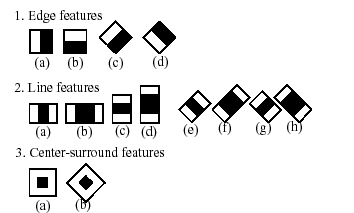
\includegraphics[width = 0.4\textwidth]{rsrc/Haarfeatures.png}
	\caption{Haar features used in openCV (including 45° features)}
	\label{fig:Haar features}
\end{figure}
The output will be the difference between the sum of the intensities on the whole picture and the intensities on the black part of the feature. The features are scaled and move across the initial image. These are quickly calculated by using the corresponding intensity image.
\begin{figure}[ht]
	\centering		
	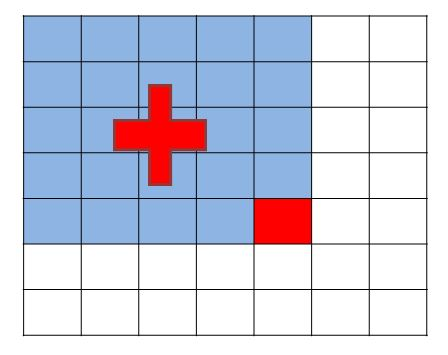
\includegraphics[width = 0.2\textwidth]{rsrc/IntegralImage.jpg}
	\caption{Integral image : sum of the intensities of the value of left and up pixels of the current pixel}
	\label{fig:Integral image}
\end{figure}
We use two intensity images, one adding the left and top pixels of the analysed pixel and an other intensity image adding the pixels in the corner of the current pixel made by two 45° lines.
The cascade is then trained. Adaboost is used for this purpose on positive images (a face, an eye, a nose, a mouth). The result is a sequences of criteria of recognition following a cascade checking of the object.
\begin{figure}[ht]
	\centering		
	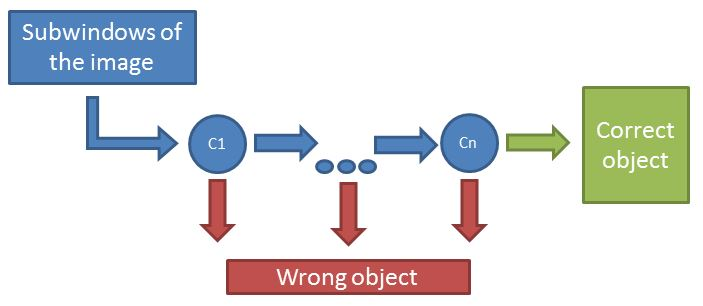
\includegraphics[width = 0.4\textwidth]{rsrc/Cascade.jpg}
	\caption{Cascade}
	\label{fig:Cascade}
\end{figure}



\subsubsection{Local Binary Pattern Histogram}

Computing of the new value of the central pixel, being the sum of powers of two combined with the value of the neighbours taken clockwise.
\begin{figure}[ht]
\centering
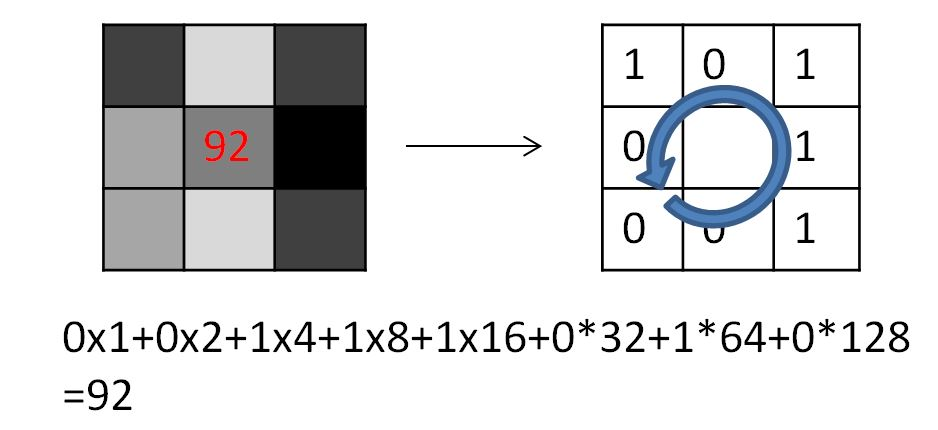
\includegraphics[width=2.5in]{rsrc/LBPH1.jpg}
\caption{Analysing the local structure}
\label{Local Structure}
\end{figure}

Addition of histograms from the subimages.

\begin{figure}[ht]
\centering
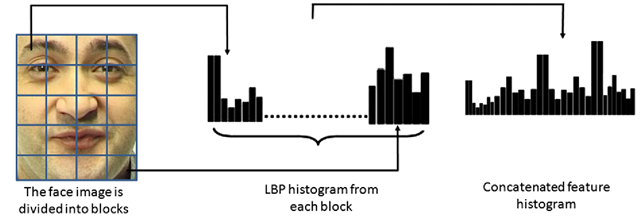
\includegraphics[width=2.5in]{rsrc/LBPH2.png}
\caption{Adding histograms (source : http://what-when-how.com/face-recognition/)}
\label{Adding histograms}
\end{figure}

%%\emph{Example of signifacance of patrial occlusion}
%%\title{Signifacance of patrial occlusion}
%%\subsection{\textbf{Signifacance of patrial occlusion}}
%%\begin{itemize}
%%	\item Eyes (occlusion of original image ~ 6\%)
%%	\item Eyebrows (occlusion of original image ~ 6\%)
%%	\item Mouth (occlusion of original image ~ 11\%)
%%	\item Eyes and nose (occlusion of original image ~ 9\%)
%%	\item Glasses (occlusion of original image ~ 15.5\%)
%%\end{itemize}




\section{Important code parts}
Appendix two text goes here.


\bibliographystyle{rsrc/IEEEtran}
\bibliography{rsrc/bibliography} % adjust this to fit your BibTex file

% that's all folks
\end{document}


